\documentclass[11pt, letterpaper]{report}

%PAQUETES A UTILIZAR
\usepackage{helvet} %PAQUETE PARA UTILIZAR LA FUENTE HELVETICA
\usepackage{graphicx} %PAQUETE QUE PERMITE LA MANIPULACIÓN DE IMAGENES
\usepackage[top=2.5cm, bottom=2.5cm, left=3cm, right=3cm]{geometry} %PAQUETE PARA MODIFICAR LOS MÁRGENES DE LA HOJA
\usepackage{fancyhdr} %PAQUETE PARA ENCABEZADOS O PIES DE PÁGINA
\usepackage{apacite} %PAQUETE QUE OFRECE EL SOPORTE PARA CITAS APA
\usepackage{parskip} %PAQUETE PARA ESPACIADO AUTOMÁTICO ENTRE PÁRRAFOS
\usepackage[compact]{titlesec} %Paquete para eliminar los espacios en blanco entre títulos, subtítulos, etc
\usepackage{setspace} %PAQUETE PARA CAMBIAR EL INTERLINEADO
\usepackage{afterpage}
%\usepackage[Lenny]{fncychap} %PAQUETE PARA CAMBIAR EL ESTILO DE TÍTULOS DE CAPÍTULOS, SECCIONES Y SUBSECCIONES
\usepackage{enumitem} %PAQUETE PARA LA CONFIGURACIÓN DE LISTAS
\usepackage{listings} %PAQUETE PARA MODIFICAR EL COMPORTAMIENTO DE LOS LISTADOS
\usepackage[bookmarks=true, pdfstartview=FitH]{hyperref} %PAQUETE PARA AÑADIR VÍNCULOS A LA TABLA DE CONTENIDOS
\usepackage{float}
\usepackage{caption} %PAQUETE PARA CONFIGURAR LOS CAPTIONS DE LAS FIGURAS.
\usepackage{config/docstyle} %PAQUETE CUSTOM PARA LA INCRUSTACIÓN DE DATOS PERSONALES
%\usepackage{showframe} %PAQUETE QUE PERMITE VISUALIZAR EL MARGEN DEL DOCUMENTO

%AQUÍ COMIENZA EL DOCUMENTO
\begin{document}
    %Referencias renombrado
\renewcommand{\bibname}{Bibliografía}

%Configurando parskip
\setlength{\parindent}{0cm}
\setlength{\parskip}{5mm}

%Configurando el espaciado entre "itemize/enumerate items"
\setlist[itemize]{noitemsep, topsep=3mm}
\setlist[enumerate]{noitemsep, topsep=3mm}

%Espacios entre autores en "Bibliografía"
\let\OLDthebibliography\thebibliography
\renewcommand\thebibliography[1]{
    \OLDthebibliography{#1}
    \setlength{\parskip}{3mm}
    \setlength{\itemsep}{3mm plus 0.3ex}
}
    \begin{titlepage}
    \begin{center}
        \begin{minipage}{0.25\textwidth} %0.15 para que quede todo en una linea
            \begin{flushleft}
                
\includegraphics[scale=0.08]{img/logo-sep-vertical.png} %scale=0.0610
            \end{flushleft}
        \end{minipage}
        \hfill
        \begin{minipage}{0.4\textwidth} %0.6 para que quede todo en una linea
            \begin{center}
                \MakeUppercase{\nombreUniversidad}
            \end{center}
        \end{minipage}
        \hfill
        \begin{minipage}{0.25\textwidth} %0.15 para que quede todo en una linea
            \begin{flushright}
                
\includegraphics[scale=0.045]{img/logo-itc.png} %scale=0.04
            \end{flushright}
        \end{minipage}
        
        \vspace{0.8cm}
        \MakeUppercase{Informe técnico de residencias profesionales}

        \nombreProyecto{}

        \vspace{0.8cm}
        \fechaInicioResidencia{} \textendash{} \fechaFinResidencia{}

        \nombreEmpresa{}

        \vspace{0.8cm}
        Presenta:

        \nombreAutor{}

        \numeroControl{}

        \especialidad{}

        \vspace{0.8cm}
        Asesor Externo

        \nombreAsesorExterno{}

        \vspace{0.8cm}
        Asesor Interno

        \nombreAsesorInterno{}

        \vspace{0.8cm}
        \fechaPresentacion{}
    \end{center}
\end{titlepage}

    \pagenumbering{Roman}
    \tableofcontents

    \newpage
    \pagenumbering{arabic}
    \chapter{Introducción}
    \chapter{Justificación}
    Mezfer es una empresa mexicana dedicada a solucionar los problemas del campo mediante la elaboración de productos dirigidos al sector agroalimentario. El creciente número de clientes llevó a Mezfer a crear ``Mezfer Rewards'', un programa de recompensas mediante el cual los clientes se inscriben a los diferentes `Programas de lealtad' para canjear puntos que reciben con la compra de productos.
    
    Actualmente, Mezfer Rewards es gestionado mediante 2 aplicaciones diferentes: 
    \begin{itemize}
        \item Una aplicación web para que los administradores puedan realizar la gestión del programa.
        \item Una aplicación móvil para que los clientes puedan realizar todo el proceso para obtener recompensas.
    \end{itemize}

    Ahora, Mezfer busca que tanto clientes como administradores puedan realizar sus respectivas actividades en una misma plataforma para así mantener un mejor control. Con este objetivo establecido, comienza el desarrollo de ``Mezfer Insider'', un portal para administradores y clientes que unifica las funcionalidades de las aplicaciones anteriores en un solo lugar.
    \chapter{Objetivos}
    \section{Objetivo General}
    \begin{itemize}
        \item Desarrollar e implementar la aplicación ``Mezfer Insider'' para centralizar y controlar las actividades de administradores y clientes.
    \end{itemize}
    \section{Objetivos específicos}
\begin{itemize}
    \item Analizar la base de datos anterior para identificar áreas de mejora.
    \item Diseñar la nueva base de datos para Mezfer Insider.
    \item Integrar Mezfer Insider a Control Manager Siso (CMS) para que los administradores puedan iniciar sesión.
    \item Crear el inicio de sesión para los clientes de Mezfer.
    \item Crear el dashboard para los clientes.
    \item Integrar la funcionalidad de canje de puntos para los clientes.
\end{itemize}
    \chapter{Problemas a resolver}
    \begin{itemize}
        \item Fragmentación de plataformas: Actualmente, el programa Mezfer Rewards es gestionado mediante dos aplicaciones separadas: una aplicación web para los administradores y una aplicación móvil para los clientes. Esta separación implica un manejo dividido e ineficiente de las funcionalidades.
        \item Descentralización: El hecho de que las actividades estén dispersas en diferentes plataformas dificulta la capacidad de mantener una visión centralizada y controlada de las operaciones.
        \item Falta de integración: Las actividades de los clientes y los administradoes están divididas en distintos sistemas, lo que hace que la gestión de tareas sea poco eficiente.
        \item Falta de adaptación de funcionalidades: Se requiere unificar las funcionalidades de las aplicaciones web y móvil en una misma plataforma. Es importante que estas funcionalidades mantengan las características clave que ofrecen, como la gestión del programa y el acceso a las recompensas.
        \item Mejora de la experiencia del usuario: El usuario es una pieza fundamental en esta nueva plataforma, por lo que es importante asegurar que tanto administradores como clientes puedan realizar sus actividades eficientemente y sin problemas para ofrecer una experiencia agradable.    
    \end{itemize}
    \chapter{Marco Teórico}
El desarrollo web es el proceso de crear y mantener sitios web y abarca una gran variedad de acciones que van desde la creación de códigos y diseños, hasta la administración de contenidos y servidores. Para el desarrollo web se utilizan diferentes lenguajes de programación que ayudan a crear el código que hace que las páginas funcionen.

Entre los lenguajes de programación más comunes para el desarrollo web se encuentran:
    \begin{itemize}
        \item HyperText Markup Language (HTML): Este lenguaje es el componente más básico de la web, y ayuda a definir el significado y la estructura del   contenido web.
        \item Cascading Style Sheet (CSS): Este lenguaje de estilos es utilizado para describir la presentación de documentos HTML o XML.
        \item Hypertext Preprocessor (PHP): Es un lenguaje de programación del lado del servidor que puede integrarse en HTML para crear aplicaciones y sitios web dinámicos.
        \item JavaScript: Es un lenguaje de programación que se ejecuta del lado del cliente de la web y es utilizado para programar cómo se comportan las páginas web cuando ocurre un evento. También puede ser ejecutado de lado del servidor, lo que permite que se puedan generar páginas web dinámicas.
    \end{itemize}
El desarrollo web se puede dividir en tres categorías: Frontend, Backend y Full Stack.

El desarrollo Frontend es el responsables de la parte del cliente, es decir, la parte que el usuario ve en pantalla cuando ingresa al sitio.

El desarrollo Backend se encarga de aspectos como servidores, bases de datos y lenguajes de programación. En esta parte se procesan las solicitudes del Frontend que contienen los datos para la base de datos u otros sitemas.

El desarrollo Full Stack es la combinación del Frontend y Backend, por lo que esta categoría es responsable tanto de la parte del cliente como de la parete del servidor.


    \chapter{Procedimiento y descripción de las actividades realizadas}
Las actividades que en esta sección son descritas están redactadas en orden cronológico y con base en el cronograma de actividades. Es importante destacar que el cronograma de actividades fue elaborado de acuerdo al tablero de actividades Kanban que se realizó para dar seguimiento a todas las actividades que se han realizado para el desarrollo del proyecto.
    \section{Conociendo Mezfer Rewards}
Mezfer Rewards es un programa de recompensas creado por la compañía Mezfer para poder entregar a sus clientes diferentes premios mediante el canje de puntos que obtienen gracias a la compra de productos. Para poder llevar a cabo este programa, Mezfer decidió crear una aplicación web y una aplicación móvil.

Para poder comenzar con el nuevo proyecto ``Mezfer Insider'' fue de gran importancia conocer ambas aplicaciones con las que funciona el proyecto, pues estas sirven como antecedentes y guías para tener una idea más sólida sobre como se va a estructurar el nuevo proyecto y todas las funciones que se van a mantener o eliminar. 

A continuación, se describen de manera general ambas aplicaciones.
    \subsection{Aplicación web de Mezfer Rewards}
La aplicación web fue desarrollada utilizando Laravel, un framework para el lenguaje de programación PHP. Esta aplicación es un pánel de administración, por lo que sólo está pensada para ser utilizada por usuarios que sean administradores. 

La aplicación está integrada a un sistema más grande llamado ``Siso ERP'', un sistema integral de gestión empresarial que controla, facilita y optimiza los procesos operativos de las empresas. Por lo tanto, para poder acceder al pánel de administración de Mezfer Rewards, es necesario tener una cuenta en Siso ERP.

Una vez que el administrador ha ingresado, podrá realizar todas las acciones necesarias para gestionar el programa. Entre las acciones más importantes se encuentran: 
\begin{itemize}
    \item Gestión de usuarios: El administrador es capaz de activar o desactivar la cuenta de un usuario, modificar su rol y suscribir o desuscribir al usuario de una campaña.
    \item Gestión de campañas: El administrador es capaz de modificar toda la información relevante de una campaña como su descripción, los productos participantes y los premios disponibles.
    \item Gestión de solicitudes de puntos: El administrador es capaz de aceptar o rechazar una solicitud de puntos que haya enviado un cliente, de acuerdo a si la evidencia que envió es válida o no. 
\end{itemize}
Hay muchas más acciones que puede realizar el administrador y que complementan al programa de recompensas. Si bien son acciones que también son importantes, no es fundamental describirlas para poder comprender mejor la aplicación.
    \subsection{Aplicación móvil de Mezfer Rewards}
La aplicación móvil fue desarrollada con Flutter, un framework que permite desarrollar aplicaciones nativas para iOS y Android, y cuyo lenguaje de programación es Dart. Esta fue desarrollada específicamente para los clientes.

Al descargar e iniciar la aplicación, los clientes deberán ingresar su número telefónico y su contraseña para acceder; si no tienen cuenta, tendrán que registrarse.

Cuando el cliente ha iniciado sesión, accederá a la aplicación y podrá ver las campañas disponibles, así como otro contenido que podría ser de su interés. Es importante mencionar que la aplicación no cuenta con una función para inscribirse a la campaña que desee, pero esto no es una falla en el diseño, sino una decisión de la propia empresa; para que el cliente pueda inscribirse tendrá que comunicarse con un encargado de Mezfer y realizar la solicitud.

Si el cliente no está inscrito a ninguna campaña, sólo podrá revisar la información general como la descripción, los productos participantes y los premios disponibles; si el cliente está inscrito a alguna campaña, además de poder ver la información general, podrá realizar dos acciones más:
\begin{itemize}
    \item Realizar solicitud de puntos: El cliente es capaz de enviar una solicitud de puntos, en donde especifica los productos que compró y la cantidad, así como la evidencia de la compra.
    \item Canjear puntos disponibles: El cliente es capaz de canjear los puntos que obtuvo con la compra de productos para poder obtener premios que sean de su interés.
\end{itemize}
Hay otras acciones que puede realizar el cliente y que complementan su experiencia en el uso de la aplicación. Si bien son acciones que también son importantes, no es fundamental describirlas para poder comprender mejor la aplicación.
    \section{Análisis de la base de datos}
    \section{Selección de tecnologías a utilizar}
Como último paso para comenzar con el desarrollo de Mezfer Insider, se analizaron diferentes tecnologías para usar en frontend y backend.
    \subsection{Servicios en la nube}
La plataforma que se utilizó para proveer los servicios en la nube fue Amazon Web Services. De esta plataforma se utilizaron servicios como:
\begin{itemize}
    \item Amazon Elastic Compute Cloud (EC2): Es un servicio que proporciona capacidad de computación escalable bajo demanda en la nube. Permite lanzar cuantos servidores virtuales sean necesarios. Dos instancias de EC2 fueron utilizadas para lanzar el proyecto de Mezfer Insider y la API.
    \item Amazon Relational Database Service (RDS): Es un servicio web que facilita la configuración, la operación y la escala de una base de datos relacional en la nube. Se utilizó este servicio para crear la base de datos de Mezfer Insider.
    \item Amazon Simple Storage Service (S3): Es un servicio de almacenamiento de objetos que ofrece escalabilidad, disponibilidad de datos, seguridad y rendimiento líderes del sector. Este servicio fue utilizado para almacenar recursos importantes de Mezfer Insider, como archivos e imágenes.
\end{itemize}
    \subsection{Tecnologías de frontend}
Para facilitar el desarrollo del frontend, se decidió comprar una plantilla de pánel de usuario llamada DashTail, la cual proporciona vistas ya diseñadas o componentes para poder ir construyendo poco a poco la vista para el usuario; esta plantilla ofrece una alta personalización, por lo que es posible realizar cualquier cambio a los componentes.

DashTail fue desarrollada utilizando Next.js y Tailwind CSS. 

Next.js es un framework basado en JavaScript y React que permite crear aplicaciones web modernas, dinámicas y escalables. Aunque es un framework full-stack, en DashTail sólo se utiliza para frontend.

Tailwind CSS es un framework de CSS para el diseño de páginas web. Su principal característica es que no genera una serie de clases predefinidas para elementos, en su lugar, crea una lista de clases ``de utilidad'' que son utilizas para dar estilos individuales a cada elemento. Es gracias a este framework que los componentes de la plantilla son altamente personalizables.
    \subsection{Tecnologías de backend}
El backend consistió en desarrollar una API para que el frontend pudiera comunicarse con esta y realizar peticiones HTTP para interactuar con la base de datos.

La principal tecnologia de backend es Node.js, un entorno de ejecución utilizado para poder ejecutar código de JavaScript directamente en los servidores, es decir, sin la necesidad de un navegador web.

Junto a Node.js se utiliza Express.js, un framework de backend para Node.js que proporciona características y herramientas robustas para desarrollar aplicaciones de backend escalables. Sus herramientas como peticiones y respuestas HTTP, enrutamiento y middlewares resultaron muy útiles para el desarrollo de la API.
    \section{Inicialización y despliegue de los proyectos de Frontend y Backend}
Para comenzar con el desarrollo de Mezfer Insider fue necesario crear los proyectos e instalar las dependencias necesarias para que estos funcionaran correctamente.
    \subsection{Inicialización del proyecto de Frontend}
Como se mencionó anteriormente, para el Frontend se utilizó una plantilla llamada DashTail, la cual proporciona un conjunto de páginas ya diseñadas. Esta plantilla es un proyecto de Next.js, por lo que, en este caso, no fue necesario crear el proyecto desde cero.

Para poder ejecutar el proyecto es necesario instalar todas las dependencias necesarias con el gestor de dependencias que se prefiera. En este proyecto se decidió utilizar el gestor de dependencias Yarn.

Cuando se instala Node.js, el gestor de dependencias predeterminado es NPM (Node Package Manager), por lo que si se desea utilizar Yarn será necesario realizar una instalación extra. En la página oficial de Yarn se explica de una manera breve y sencilla como se realizar la instalación; utilizando NPM se ejecuta el siguiente comando:
    \begin{center}
        \textbf{
            \emph{
                npm install --global yarn
                }
            }
    \end{center}
De esta manera Yarn quedará instalado en todo el sistema y podrá ser utilizado en cualquier proyecto.

Ahora, lo único que queda es instalar las dependencias del proyecto. Para esto, se ejecuta el comando: 
    \begin{center}
        \textbf{
            \emph{
                yarn install
                }
            }
    \end{center}
Y con esto comenzará la instalación.

Una vez instaladas todas las dependencias, se ejecuta el comando:
    \begin{center}
        \textbf{
            \emph{
                yarn dev
                }
            }
    \end{center}
Esto iniciará el entorno de desarrollo del proyecto, que será ejecutado en un servidor local y para acceder a él simplemente en un navegador escribimos la URL \emph{http://localhost:3000} (El puerto 3000 es el puerto predeterminado en el cual se ejecuta el servidor local de Next.js, sin embargo, este puede ser cambiado al puerto que se desee).
    \subsection{Despliegue del proyecto de Frontend en servidor de producción}
Para desplegar el proyecto en el servidor de producción se deben seguir casi los mismos pasos que con la inicialización, pero hay algunos pasos extra que deben realizarse.

Principalmente, deben de estar instalados Node.js y Yarn para poder instalar las dependencias y ejecutar el proyecto. El proceso de instalación es el mismo, no hay ninguna diferencia.

Otra herramienta importante que se debe instalar es PM2 (Process Manager 2), un gestor de procesos que permite mantener proyectos de Node.js en ejecución, es decir, si el servidor llegase a ser detenido o reiniciado, PM2 se encargará de iniciar el proyecto automáticamente sin la necesidad de que un administrador ingrese al servidor a iniciar todos los proyectos nuevamente. Para instalar PM2, se ejecuta el siguiente comando:
    \begin{center}
        \textbf{
            \emph{
                yarn global add pm2
                }
            }
    \end{center}
El siguiente paso es compilar el proyecto para que Next.js realice todas las optimizaciones necesarias y así quede preparado para producción. Para compilar el proyecto, desde la carpeta principal se ejecuta el siguiente comando:
    \begin{center}
        \textbf{
            \emph{
                yarn build
                }
            }
    \end{center}
De esta manera Next.js comenzará a compilar y optimizar todas las páginas que tenga la aplicación. Al finalizar el proceso, se creará una carpeta llamada ``.next'', la cual contiene el proyecto optimizado y listo para producción.

Ahora, hay 5 archivos importantes que deben ser enviados al servidor para poder ejecutar correctamente el proyecto:
    \begin{itemize}
        \item .next: Esta es la carpeta que contiene todo el proyecto optimizado.
        \item .env: Este es el archivo donde se almacenan las variables de entorno.
        \item package.json: Este es el archivo que contiene todas las dependencias que han sido instaladas en el proyecto.
        \item yarn.lock: Un archivo generado por Yarn que lleva un registro de las versiones exactas de las dependencias que requiere un proyecto para que funcione adecuadamente.
        \item next.config.js: Este es el archivo que contiene la configuración del servidor de Next.js.
    \end{itemize}
Para enviar estos archivos al servidor, se ejecuta el siguiente comando:
    \begin{center}
        \textbf{
            \emph{
                scp -i --/ruta/llave/PEM -r archivos usuario@ip\_{}publica\_{}servidor:--/carpeta/destino
                }
            }
    \end{center}
Una vez estén todos los archivos en el servidor de producción, se instalan las dependencias como se explicó anteriormente, y finalmente, se ejecuta el proyecto con PM2 para que este se encargue de gestionarlo. Para ejecutar el proyecto con PM2, se utiliza el siguiente comando:
    \begin{center}
        \textbf{
            \emph{
                pm2 start ``yarn start'' --name nombre-app
                }
            }
    \end{center}
Posteriormente, se guarda la configuración con el siguiente comando:
    \begin{center}
        \textbf{
            \emph{
                pm2 save
                }
            }
    \end{center}
Para hacer que la aplicación se ejecute automáticamente cuando se reinicie el servidor, se utiliza el siguiente comando:
    \begin{center}
        \textbf{
            \emph{
                pm2 startup
                }
            }
    \end{center}
Al ejectuar este comando PM2 proporcionará otro comando que solamente debe ser copiado, pegado y ejecutado, y se habrá terminado de configurar. Ahora, con cada reinicio del servidor, la aplicación se ejecutará automáticamente.

Cuando se quieran subir cambios al proyectos, simplemente se repiten los pasos:
    \begin{itemize}
        \item Compilar el proyecto.
        \item Subir los archivos que hayan sufrido cambios al servidor.
        \item Reiniciar el proceso de PM2.
    \end{itemize}
Para reiniciar el proceso de PM2, se ejecuta uno de los siguientes comandos:
    \begin{center}
        \textbf{
            \emph{
                pm2 reload nombre-app
                }
            }

        \textbf{
            \emph{
                pm2 restart nombre-app
            }
        }
    \end{center}
Y con esto quedarán aplicados los cambios que se hayan subido.
    \subsection{Inicialización del proyecto de Backend}
El proyecto de Backend consiste en una API realizada en el framework Express.js. Este proyecto sí es creado desde cero, por lo que se deben seguir unos cuantos pasos extra. Es importante mencionar que también debe estar ya instalado Node.js, al igual que un gestor de dependencias.

Lo primero que se tiene que hacer es crear una carpeta donde va a estar guardado todo el proyecto. Para crear una carpeta, se ejecuta el siguiente comando (puede cambiar de acuerdo al Sistema Operativo que se use):
    \begin{center}
        \textbf{
            \emph{
                mkdir nombre-carpeta
                }
            }
    \end{center}
Posteriormente, se ingresa a la carpeta y desde ahí se ejecuta el siguiente comando:
    \begin{center}
        \textbf{
            \emph{
                npm init -y
                }
            }
    \end{center}
Lo que hace ese comando es iniciar la configuración del proyecto, al usuario se le hacen ciertas preguntas para saber que cosas quiere incluir o usar. La opción -y hace que a todas las preguntas se les responda con un ``sí'', por lo que se puede omitir si se desea pensar un poco más en la configuración.

Como esta es una API realizada con Express.js, es necesario instalar el paquete. Para instalar Express.js, se ejecuta el siguiente comando:
    \begin{center}
        \textbf{
            \emph{
                npm install express
                }
            }
    \end{center}
Ahora sólo falta crear el servidor de Express, ya que ahí es donde se realizarán las diferentes solicitudes HTTP desde el Frontend. Para lograr esto, se crea un archivo que preferentemente se llame ``index.js'', aunque puede llevar cualquier nombre; en este archivo es donde se inicializa el servidor y se colocan las rutas y middlewares que vayan a ser ocupados. Para inicializar el servidor de Express, se añaden las siguientes líneas de código (Ver figura 1):

    \begin{figure}[H]
        \begin{center}
            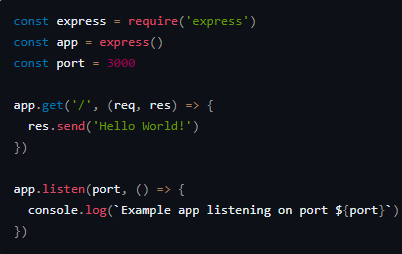
\includegraphics[scale=0.84]{img/actividades/inicializacion-despliegue/express-basic-app.png}
            \caption{Aplicación básica de Express.}
            \label{fig:express-basic-app}
        \end{center}
    \end{figure}
Y para ejecutar la aplicación, se utiliza el siguiente comando:
    \begin{center}
        \textbf{
            \emph{
                node index.js
                }
            }
    \end{center}
Con ese comando se ejecuta el servidor de manera local y se pueden realizar algunas solicitudes HTTP a la URL \emph{http://localhost:3000}.
    \subsection{Despliegue del proyecto de Backend en servidor de producción}
La estrategia que se siguió para desplegar la API en el servidor de producción fue utilizar repositorios de GitHub, ya que estos es posible clonarlos en cualquier parte y esto facilita y simplifica el proceso de despliegue.

Lo primero que se debe hacer es crear un repositorio de GitHub. Esto se puede hacer desde la línea de comandos o desde la página web, pero para más facilidad se recomienda realizarlo desde la página web. Una vez creado el repositorio, se proporcionan una serie de comandos que se deben ejecutar para inicializar el repositorio local y subir el código ya existente al repositorio remoto.

Una vez que el código se encuentre en el repositorio remoto sigue clonarlo en el servidor de producción. Realizar la clonación de un repositorio es muy sencillo, sólo es necesario ingresar al servidor y ubicarse en el directorio donde va a estar el proyecto, luego se ejecuta el siguiente comando: 
    \begin{center}
        \textbf{
            \emph{
                git clone ruta-del-repositorio-remoto
                }
            }
    \end{center}
Y con esto todas las carpetas y archivos del proyecto estarán en el servidor de producción. Después, se deben instalar todas las dependencias mediante el siguiente comando:
    \begin{center}
        \textbf{
            \emph{
                npm install 
                }
            }
    \end{center}
El último paso es hacer que se ejecute automáticamente la aplicación, y esto se logra gracias a PM2. Los comandos que se utilizan son prácticamente los mismos, sólo hay una ligera variación en el primer comando que se utiliza, puesto que ejectuar una aplicación de Express es diferente a ejecutar una aplicación de Next.js. El comando que se debe usar para esta aplicación es el siguiente:
    \begin{center}
        \textbf{
            \emph{
                pm2 start ``node index.js'' --name nombre-app
                }
            }
    \end{center}
Los siguientes comandos a ejecutar son exactamente los mismos que se explicaron en el despliegue de la aplicación del Frontend.

Para actualizar la aplicación, simplemente se suben los cambios realizados en el código al repositorio remoto y se descargan en el servidor de producción mediante el siguiente comando:
    \begin{center}
        \textbf{
            \emph{
                git pull
                }
            }
    \end{center}
Una vez descargados los cambios, se reinicia el proceso de PM2 y la aplicación ya estará en su última versión.
    \section{Creación de balanceadores de carga y asignación de los dominios}
    \section{Integración de Mezfer Insider con Control Manager Siso}
Control Manager Siso (CMS) es el sistema de inicio de sesión de Siso ERP, un sistema ERP que permite realizar la gestión de distintos aspectos de una empresa. Cuando un cliente compra una licencia de Siso ERP, se le otorgan un correo y contraseña que podrán usar para iniciar sesión mediante CMS y acceder a sus empresas.

Quienes son administradores de CMS tienen acceso al panel de administración, donde se les permite gestionar a los usuarios y empresas del sistema Siso ERP.

Para poder crear empresas (que son tratadas como aplicaciones web), CMS realiza peticiones a diferentes endpoints de la API de la nueva empresa y, dependiendo de la respuesta que se reciba, se registrará correctamente a la base de datos o no. Lo mismo aplica para cuando se quiere asignar un usuario a una empresa y cuando se quiere ingresar a la empresa.
    \subsection{Creación de endpoints en la API de Mezfer Insider}
En la API de Mezfer Insider deben existir tres endpoints que permitirán a CMS realizar las acciones necesarias para registrar el proyecto en su base de datos.

El primer endpoint consiste en que se procese la información de la empresa. Mediante el Frontend, el administrador ingresa la información de la empresa en el formulario correspondiente y esta es enviada a la API; dependiendo de las necesidades del proyecto, esta información puede ser procesada o solamente recibida. En el caso de Mezfer Insider, esta información no requiere ser almacenada ni requiere ser procesada. Se debe retornar una respuesta con el código de estado de respuesta HTTP 202, indicando así que la petición se ha recibido, pero no se ha actuado.

El segundo endpoint consiste en vincular a un usuario con la empresa para indicar al sistema que ese usuario va a poder acceder a la empresa. En CMS, el administrador se encargará de asignarle la empresa al usuario, lo que enviará una nueva petición a la API para permitir la vinculación. La API recibirá el usuario y la empresa que están siendo vinuclados, esta información será procesada de acuerdo a las necesidades del proyecto. La API enviará un código de estado de respuesta HTTP 200, indicando que la operación ha sido realizada con éxito.

El tercer endpoint permitirá al usuario acceder a la empresa. Este endpoint es un poco más complejo, pues requiere el procesamiento de tokens JWT. Cuando el usuario ingresa en la empresa, CMS envía en la URL un token JWT con cierta información del usuario.
Para Mezfer Insider, esta información es importante pues se considera que todos los usuarios que ingresen mediante CMS son administradores, así que debe de quedar registro de ellos. Cuando se recupera el token de la URL, este es decodificado y se lee cierta información que posteriormente es utilizada para realizar otra petición a la API de CMS y así obtener la información completa del usuario; con esto se crea un objeto con la información que se requiere del usuario para guardarla en la base de datos. Una vez guardado el usuario, se procede a crear un token JWT propio de Mezfer Insider que posteriormente será almacenado en una cookie, de esta manera se creará una cookie de sesión que será de utilidad para permitir al usuario realizar distintas acciones dentro de la aplicación. Este proceso se repite cada que un usuario ingresa a la empresa, por lo que debe validarse la existencia del usuario en la base de datos para evitar que se intente guardar nuevamente.
    \subsection{Creación de la empresa, vinculación del usuario e ingreso}
Con los endpoints creados, ya es posible realizar todas las acciones necesarias para integrar Mezfer Insider con CMS.

Lo primero que se tiene que hacer es crear la empresa, y para eso se llena un formulario con todos los datos de la empresa.
    \begin{figure}[H]
        \begin{center}
            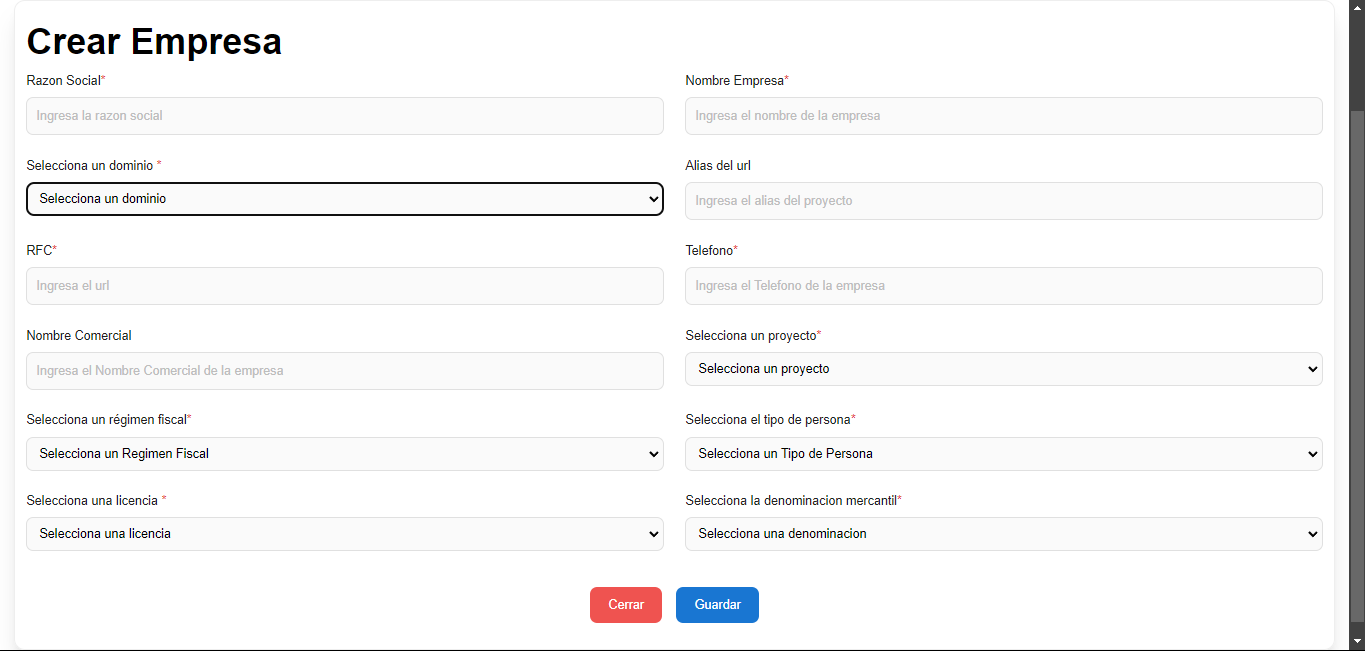
\includegraphics[scale=0.4]{img/actividades/integracion/formulario-empresa.png}
            \caption{Formulario para la creación de empresa.}
            \label{fig:formulario-empresa}
        \end{center}
    \end{figure}
Posteriormente, el usuario debe ser vinculado con la empresa.
    \begin{figure}[H]
        \begin{center}
            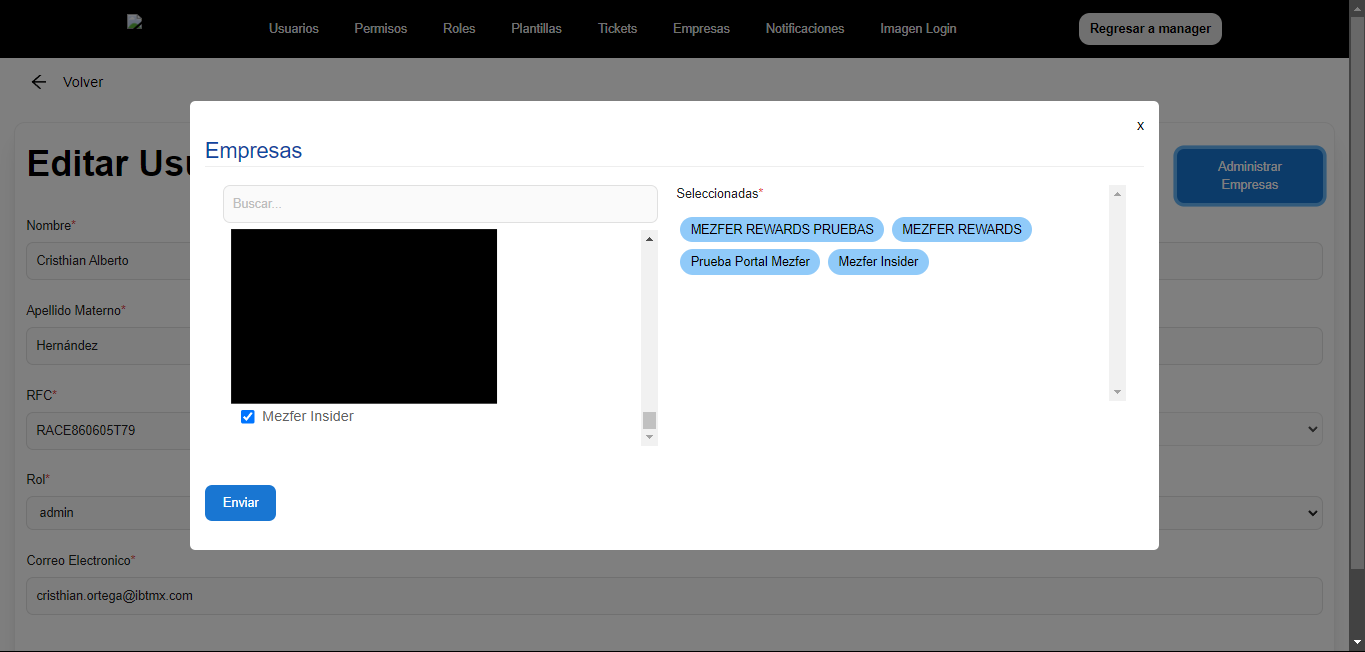
\includegraphics[scale=0.4]{img/actividades/integracion/vincular-usuario.png}
            \caption{Vinculación de usuario con empresa.}
            \label{fig:vincular-usuario}
        \end{center}
    \end{figure}
Y con esto realizado, el usuario ya podrá tener acceso a la empresa.
    \begin{figure}[H]
        \begin{center}
            
\includegraphics[scale=0.4]{img/actividades/integracion/ingreso-empresa.png}
            \caption{Selección de empresa.}
            \label{fig:ingreso-empresa}
        \end{center}
    \end{figure}
    \section{Creación de conexiones a las bases de datos}
Para poder empezar a codificar todas las acciones que se podrán realizar en Mezfer Insider, es necesario que en el backend estén realizadas las conexiones a las bases de datos para poder recuperar y guardar información.

Se realizaron dos conexiones puesto que, hasta el momento de la redacción de este reporte, Mezfer Insider ocupaba tanto la antigua base de datos como la nueva.
    \subsection{Instalación de librería}
Para poder realizar las conexiones a las bases de datos es necesario instalar una librería que proporcione los módulos del Sistema Gestor de Bases de Datos.

La librería que se seleccionó para este proyecto fue Knex.js, un constructor de queries de código abierto para JavaScript. Knex.js tiene soporte para varios SGBD, incluído PostgreSQL, que es el que se utiliza.

Para instalar Knex.js, se ejecuta el siguiente comando dentro de la carpeta del proyecto:
    \begin{center}
        \textbf{
            \emph{
                npm install knex
                }
            }
    \end{center}
    \subsection{Configuración de conexiones}
Con Knex.js instalado, sólo falta configurar las conexiones.

Para realizar las configuraciones, se debe crear un archivo que lleve de preferencia el nombre ``knexfile.js''. En este archivo, se crea un objeto con las siguientes propiedades:
    \begin{itemize}
        \item alias: El nombre que se le dará a la conexión.
        \item client: El SGBD que se utilizará para realizar la conexión.
        \item connection: En esta propiedad se debe configurar lo siguiente:
            \begin{itemize}
                \item host: El servidor donde está almacenada la base de datos.
                \item port: El puerto donde se está ejecutando el SGBD.
                \item database: El nombre de la base de datos.
                \item user: El nombre del usuario dueño de la base de datos.
                \item password: La contraseña para acceder a la base de datos.
            \end{itemize}
        \item pool: En esta propiedad se debe configurar lo siguiente:
            \begin{itemize}
                \item min: El número mínimo de conexiones que se pueden realizar.
                \item max: El número máximo de conexiones que se pueden realizar.
                \item afterCreate: Una función que se ejecuta una vez realizada la conexión. Esta es opcional
            \end{itemize}
    \end{itemize}
La estructura del objeto queda de la siguiente manera (Ver Figura 5):
    \begin{figure}[H]
        \begin{center}
            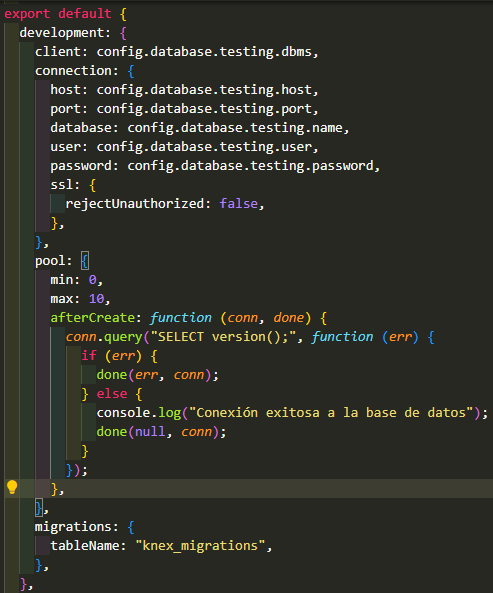
\includegraphics[scale=0.6]{img/actividades/conexion/objeto-conexion.png}
            \caption{Estructura del objeto de configuración de la conexión.}
            \label{fig:estructura-objeto}
        \end{center}
    \end{figure}
Por último, se crea una instancia de Knex y se le asigna la configuración que se desea utilizar, de esta manera se creará la conexión y se podrán realizar los queries que se requieran.
    \section{Inicio de sesión para Mezfer Insider}
El ingreso a Mezfer Insider se puede hacer de dos maneras: como cliente o como administrador.

En esta sección se explicará cómo se desarrollo el inicio de sesión de ambos roles.
    \subsection{Inicio de sesión de administradores}
Anteriormente se explicó una actividad donde se integraba Mezfer Insider a CMS. Esta integración, además de permitir la creación de la empresa en el sistema, también permite el inicio de sesión de los administradores pues todas las personas que ingresen a Mezfer Insider desde CMS son consideradas con ese rol.

Explicar como se realizó el inicio de sesión de administradores sería redundante, pues esto ya se explicó anteriormente. Para conocer este proceso, puede leer la sección 6.6 de este reporte.
    \subsection{Inicio de sesión de clientes}
Para la creación del inicio de sesión de clientes se realizaron actividades en el Frontend y en el Backend.
    \input{lib/desarrollo/act-realizadas/login/cliente/endpoint/endpoint.tex}
    \input{lib/desarrollo/act-realizadas/login/cliente/formulario-login/formulario.tex}
    \section{Dashboard del cliente}
Hasta el momento de la redacción de este reporte, el dashboard del cliente sólo muestra un saludo personalizado y las campañas activas de Mezfer.
    \subsection{Endpoints del backend para el dashboard}
Para poder mostrar el contenido correcto en el dashboard, primero es necesario obtenerlo de la base de datos. Para ello, se crearon dos endpoints en la API.
    \input{lib/desarrollo/act-realizadas/dashboard-cliente/backend/endpoints/endpoint-campanias.tex}
    \input{lib/desarrollo/act-realizadas/dashboard-cliente/backend/endpoints/endpoint-usuarios.tex}
    \subsection{Interfaz del Dashboard}
Al iniciar sesión, la primera página que ve el cliente es el dashboard. En este dashboard se muestra un mensaje personalizado para el cliente y las campañas activas de Mezfer (Ver Figura 7).

    \begin{figure}[H]
        \begin{center}
            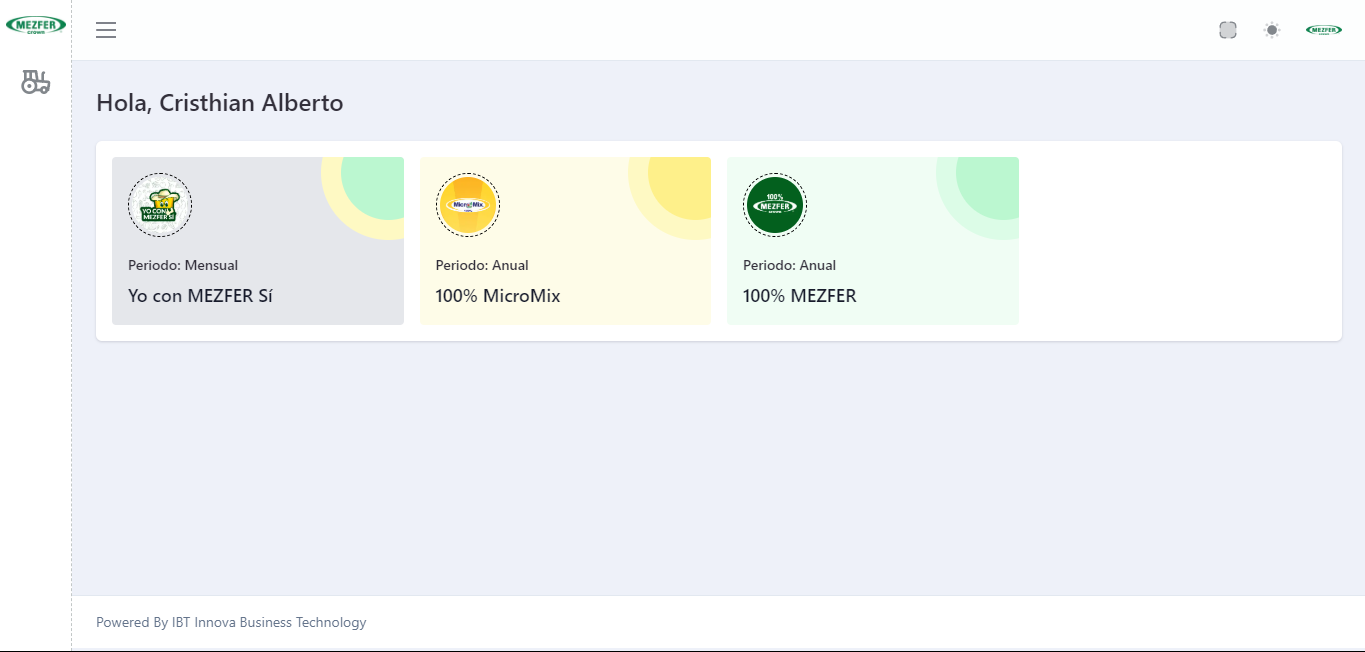
\includegraphics[scale=0.35]{img/actividades/dashboard-cliente/dashboard-cliente.png}
            \caption{Dashboard de clientes.}
            \label{fig:dashboard-clientes}
        \end{center}
    \end{figure}

Antes de cargar las campañas y el mensaje personalizado, se renderiza un componente llamado ``Skeleton'' que muestra la estructura de la página pero sin ningún contenido, sólo elementos grises que representan que la información se esta cargando. Este componente se muestra en lo que se obtiene la información de la API.

Una vez se haya cargado la información, el Skeleton deja de renderizarse y ahora muestra el mensaje personalizado y las campañas activas en componentes llamados ``Cards''. El cliente puede dar clic a cada una de estas Cards, lo que lo llevará a otra página donde se muestran todos los detalles de la campaña, pero esto se explicará más adelante.
    \section{Sección ``Mis campañas''}
La sección de campañas tiene un diseño muy similar al dashboard del clientes, lo que las hace diferentes es que la sección de campañas muestra en cuales se encuentra inscrito el usuario.
    \subsection{Endpoints del backend de la sección ``Mis campañas''}
La sección de campañas sólo requiere de dos endpoints: uno para obtener las campañas activas y otro para obtener las camapañas en las que está inscrito el usuario.
    \input{lib/desarrollo/act-realizadas/campanias/backend/endpoints/endpoint-campanias.tex}
    \input{lib/desarrollo/act-realizadas/campanias/backend/endpoints/endpoint-inscrito.tex}
    \subsection{Interfaz de la sección ``Mis campañas''}
En la parte izquierda de la página web, el usuario podrá ver una barra de navegación que contiene un ícono de un tractor. Al dar clic en este tractor, el usuario será dirigido a la sección ``Mis campañas''.

En esta sección también se utiliza el componente ``Skeleton'' para indicar que se está cargando la información.

Cuando se cargan la información, el Frontend recibe todas las campañas activas y las campañas en las que se encuentra inscrito el usuario. Antes de construir la interfaz, se realiza un filtrado de los resultados obtenidos. Dentro del arreglo que contiene las campañas activas se buscan coincidencias con el arreglo que contiene las campañas en las que está inscrito el usuario; las campañas que se encuentren en ambos arreglos se almacenan en un nuevo arreglo, y las que no coincidan se ignoran.

Este nuevo arreglo es el que se utiliza para renderizar las Cards de las campañas, y de esta manera sólo se le muestran al usuario sus campañas correspondientes (Ver Figura 8).

    \begin{figure}[H]
        \begin{center}
            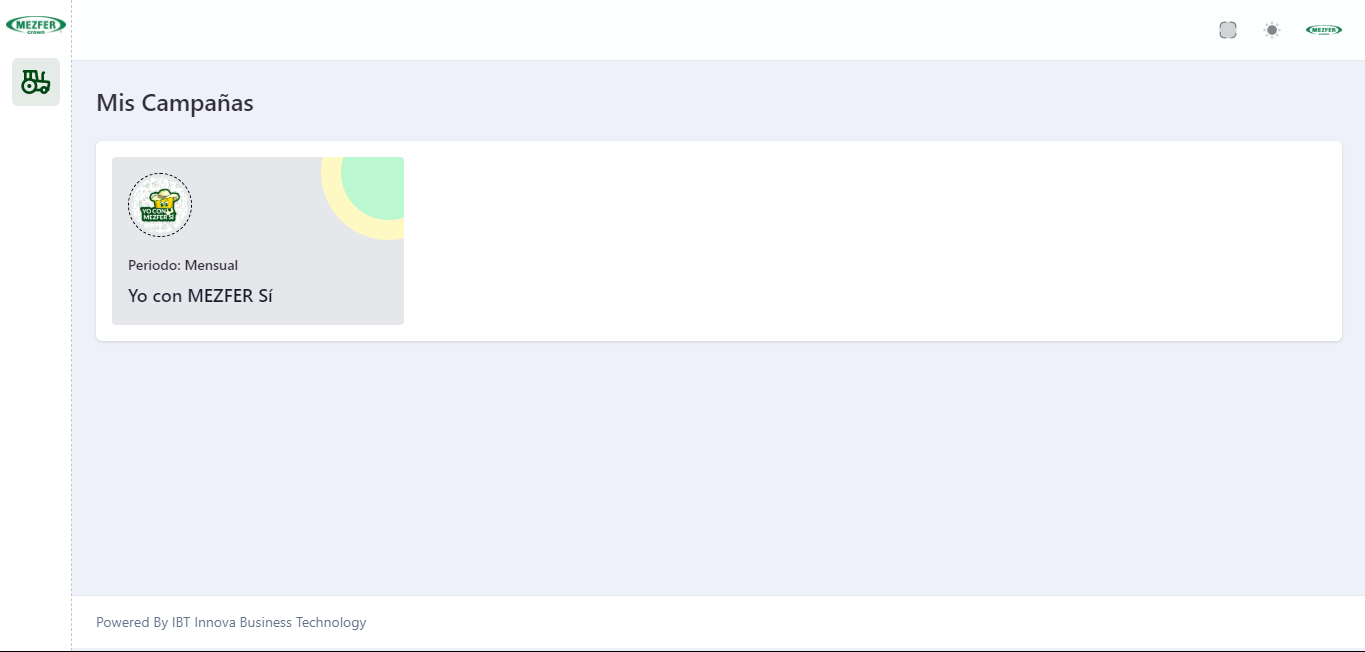
\includegraphics[scale=0.35]{img/actividades/campanias/mis-campanias.png}
            \caption{Sección ``Mis campañas''.}
            \label{fig:seccion-campañas}
        \end{center}
    \end{figure}
    \section{Detalles de las campañas}
Esta es una subsección de la sección de campañas. Aquí los usuarios podrán ver toda la información específica de una campaña.
    \subsection{Endpoints del backend de la sección ``Detalles de las campañas''}
Esta sección requiere de una cantidad mayor de endpoints debido a toda la información que se debe obtener para poder mostrarla a los usuarios.
    \input{lib/desarrollo/act-realizadas/campanias-detalles/backend/endpoints/endpoint-campania-info.tex}
    \input{lib/desarrollo/act-realizadas/campanias-detalles/backend/endpoints/endpoint-inscrito.tex}
    \input{lib/desarrollo/act-realizadas/campanias-detalles/backend/endpoints/endpoint-premios.tex}
    \input{lib/desarrollo/act-realizadas/campanias-detalles/backend/endpoints/endpoint-productos.tex}
    \input{lib/desarrollo/act-realizadas/campanias-detalles/backend/endpoints/endpoint-solicitudes.tex}
    \input{lib/desarrollo/act-realizadas/campanias-detalles/backend/endpoints/endpoint-canjes.tex}
    \input{lib/desarrollo/act-realizadas/campanias-detalles/backend/endpoints/endpoint-puntos.tex}
    \input{lib/desarrollo/act-realizadas/campanias-detalles/backend/endpoints/endpoint-solicitud-puntos.tex}
    \subsection{Interfaz de la sección ``Detalles de las campañas''}
Anteriormente se había mencionado que las Cards donde se mostraban las campañas, cuando el usuario hace clic en ellas, dirigían a una nueva página. Esta nueva página es la sección donde el usuario puede leer toda la información de la campaña que haya seleccionado.

Debido a que esta sección es un poco más grande que otras que se han descrito, se va a separar en dos: el encabezado de la sección y el contenido.

Al igual que en secciones anteriores, mientras se está cargando la información se renderiza el componente ``Skeleton''. Una vez cargada la información, se muestra el contenido normal de la página.
    \input{lib/desarrollo/act-realizadas/campanias-detalles/frontend/encabezado/encabezado.tex}
    \input{lib/desarrollo/act-realizadas/campanias-detalles/frontend/contenido/contenido.tex}
    \section{Cambios generales en el Frontend de los clientes}
Los cambios que se realizaron en el Frontend de los clientes son relacionados al código y a algunos componentes.

En cuanto al código, se cambió la manera en las que se estaban realizando las peticiones HTTP. Las peticiones se estaban realizando de manera repetida en diferentes partes del código, por lo que se decidió realizarlas desde un mismo lugar y la información que se obtuviera se pasaría a los diferentes componentes que la necesitaran. Además, como la misma estructura de código se repetía, se decidió crear un hook para realizar las peticiones; ahora en vez de escribir el mismo código múltiples veces, simplemente se manda a llamar un método que solicita una URL y el tipo de petición.

Otro cambio importante que se realizó fue en los componentes. Algunos componentes como tablas, Dialogs y Cards se estaban creando por cada sección que los ocupara y esto sólo hacía que el tamaño del proyecto estuviera aumentando, es por eso que se decidió crear componentes reutilizables, esto permitió que en un solo archivo estuviera el códgio general de cada componente y sólo se les pasaba la información que se quisiera mostrar en ellos.


    \input{}
    
\end{document}